\documentclass[a4paper, sigconf]{acmart}
\usepackage{multirow,hhline,graphicx,array}
\usepackage{fullwidth}
\usepackage{framed}
\newcolumntype{M}[1]{>{\centering\arraybackslash}m{#1}}

\title{Black-Box Transformation of the GASLITE Attack}
\author{Ishay Yemini\\Tel Aviv University\\ \today}
\date{\today}

\settopmatter{printacmref=false}
\setcopyright{none}
\renewcommand\footnotetextcopyrightpermission[1]{}
\pagestyle{plain}

\begin{document}

\maketitle

\section*{Abstract}

Retrieval-Augmented Generation (RAG) systems are increasingly vulnerable to adversarial attacks that manipulate their retrieval components. However, many state-of-the-art attacks require white-box access to model gradients, an assumption that is often unrealistic in practice. This project introduces the Combination Attack, a novel and highly effective black-box attack on dense retrieval models. My method employs a two-stage optimization strategy: it first uses a random search to generate a promising initial adversarial passage, which is then refined using a robust, block-based optimization algorithm inspired by the Square Attack. I evaluate my attack on the MSMARCO dataset against a diverse suite of nine modern sentence-transformer models. The results demonstrate that the Combination Attack significantly outperforms existing black-box baselines. Most notably, it achieves top-1 retrieval success rates of over 90\% for most models, demonstrating performance remarkably close to that of the state-of-the-art white-box attack, GASLITE. This work shows that the performance gap between black-box and white-box attacks is smaller than previously assumed, highlighting a practical and potent security vulnerability in modern RAG systems that rely on model obscurity for defense.


\section{Introduction}

Retrieval-augmented generation (RAG) systems are becoming more and more common in various natural language processing applications. This has led to a rise in research dedicated to understanding and mitigating their vulnerabilities to adversarial attacks. These attacks aim to degrade the performance of RAG systems, often by manipulating the retrieval component. However, many existing attack methods operate under the assumption of white-box access, implying that the attacker has complete knowledge of the RAG system's internal mechanisms, including its parameters and gradients. This assumption is often unrealistic in real-world scenarios, where attackers typically lack such privileged access. 

GASLITE is one such attack that, based on its nature of manipulating embeddings through gradient information, requires direct access to the gradients of the dense retrieval model. To address the limitations imposed by white-box requirements, this project seeks potential methods and research directions for transforming the GASLITE attack into a black-box attack. The focus will be on techniques that can bypass the need for direct gradient access, thereby enhancing the practicality and applicability of adversarial attacks against dense retrieval systems in more realistic threat models.


\section{Related Work}

\subsection{GASLITE}

GASLITE is a newly proposed attack method to agains embedding-based RAGs \cite{bentov2024}. 
GASLITE uses a gradient-based search method in order to generate adversarial passages for promoting a chosen malicious passage, without modifying the model or relying on the specific corpus content. 
By carefully crafting perturbations to add on top of the selected poison, GASLITE can promote it to the top of the retrieval list for specific queries \cite{bentov2024}.

In this paper, the researches focused on three types of attacks: Knows All, where the attacker knows the specific query to be attacked, in which case they consistently managed to make the crafted passages be the top-1 result; Knows What, targeting a concept and not a specific query, where they also achieved impressing results, managing the promote the poison to the top-10 for most queries and most models; and Knows Nothing, for concept agnostic attacks, which they found to be the most challenging but still achieved top-10 visibility for more than 10\% of queries \cite{bentov2024}.
 
Still, the fundamental limitation of GASLITE, which I seek to improve on in my research, is its requirement for direct access to the model's gradients. This limits the attack to White-Box scenarios only, a limit that is often not met in practical settings where RAG systems are deployed as black boxes with none (or limited) access to their gradients and internal workings \cite{bentov2024}. 


\subsection{CorruptRAG}

Zhang et al. propose CorruptRAG, a poisoning attack designed for practicality and stealth \cite{zhang2025}. The key innovation of CorruptRAG is its ability to succeed by injecting only a single poisoned document into the knowledge base, whereas other methods often required multiple injections to ensure retrieval. 

The attack's primary goal is to corrupt the final generated answer of the RAG system, which it achieves through two distinct strategies: "Answer Suppression," which aims to prevent the LLM from finding the correct answer in the retrieved context, and "Answer Knowledge Corruption," which subtly misleads the LLM into trusting the incorrect information provided in the poisoned document \cite{zhang2025}.

While my Combination Attack also operates with a single document, its objective and evaluation are focused on maximizing retrieval rank. In contrast, CorruptRAG's techniques are centered on linguistic manipulation to influence the LLM's reasoning, with its success being measured by the incorrectness of the final generated output. Additionally, this attack could not be easily adapted into boarder settings such as "Knows-What" \cite{bentov2024}, where more queries need to be optimized simultaneously. 


\subsection{PoisonedRAG}

Zou et al. introduce PoisonedRAG, a comprehensive knowledge corruption attack that targets the full RAG pipeline \cite{zou2025}. Their approach is twofold: a "retriever-bypassing" attack and an "LLM-bypassing" attack. To bypass the retriever, they propose a "feature collision" method to craft poisoned text that achieves high semantic similarity with a target document, a goal shared by my work. 

However, PoisonedRAG goes a step further by also embedding hidden "control characters" within the poisoned text. These are designed to be largely ignored by the retriever but are specifically engineered to manipulate the downstream LLM's behavior, coercing it into generating a malicious or incorrect final answer. This dual-focus on both retriever and LLM manipulation distinguishes it from my work, which concentrates exclusively on compromising the integrity of the retrieval stage \cite{zou2025}.


\subsection{Square Attack}

Andriushchenko et al. \cite{andriushchenko2020} introduce the Square Attack, a query-efficient black-box adversarial attack. The method utilizes a randomized search approach that applies localized, square-shaped perturbations to an image. The attack starts with a pre-defined square size, chooses a random area to attack, and then on each iteration the square's area gets smaller. This strategy allows the attack to be much faster and efficient than random search, as it counts not just a single pixel but an entire area. The authors managed to demonstrate that the Square Attack can even outperform some white-box attacks on standard benchmarks, and is capable of breaking defenses that appear robust to traditional PGD attacks. 


\subsection{Universal Adversarial Triggers}

My main direction to explore was the idea of Universal Adversarial Triggers (UATs) \cite{wallace2021}. This idea relates to the concept of manipulating text embeddings through certain token sequences. Specifically, UATs are a sequence of tokens that, when appended to any input text, can cause a ML model to produce an incorrect or targeted prediction. The work in this area introduces gradient-guided methods for discovering these triggers. While the process for finding UATs often relies on having white-box access to the model, the resulting UATs are input-agnostic and have been shown to sometimes transfer affectively to other models, even with different embeddings and architectures \cite{wallace2021}.

UATs have been shown to demonstrate potential in attacking the safeguards of LLMs \cite{liang2025}. UATs might achieve this effect by approximating semantic information within their adversarial training region \cite{subhash2023}. This implies that the manipulation cause by UATs may not be arbitrary, but could be related to semantically meaningful directions in the embedding space, similar to the embedding manipulation goals of the GASLITE attack \cite{bentov2024}. Therefore, I wanted to explore the possibility of finding UATs that, when appended to queries or documents, can manipulate the retrieval rankings in dense retrieval models without direct access to the gradients. This transferability property of UATs, where a trigger found from a surrogate model and might also work on the target dense retriever, is especially relevant for my black-box goal. 


\section{Technical Approach}


The approach of my attack evolved significantly through an ever-changing process of experimentation, analysis, and refinement, starting with a simple, random algorithm and moving towards a more sophisticated, two-stage attack strategy. 

My goal was to develop a black-box attack, capable of manipulating the retrieval ranking for a given query, with the same threat model as the "Knows-All" setting from the GASLITE paper \cite{bentov2024}. This setting assumes the attacker knows the target query, and can craft a specific suffix to a random malicious passage \texttt{info}, to turn it into an adversarial passage. 


\subsection{Random Search Attack}

The first iteration of the attack was a simple, greedy, token-by-token random search, implemented in the \texttt{random\_attack} method. The logic was simple: 

\begin{enumerate}
  \item Start with a base "poison".
  \item At each step, generate a pool of several hundred random candidate tokens from the model's vocabulary. 
  \item For each candidate token, calculate the cosine similarity when temporarily appending it to the current passage.
  \item Select the token that yields the highest similarity score, permanently append it to the passage, and proceed to the next step.  
\end{enumerate}

This simple attack showed some promising success with certain passages from MSMARCO using the E5 model, however when generalized to a 50-query trial in the same setting as GASLITE \cite{bentov2024}, the attack's success became minimal, managing to bring the poison to the top result of the query only once.


\subsection{Query Stuffing}

As a temporary improvement, I made an enhancement to the random attack by first appending the text of the target query directly to the end of the poison passage, before running the attack. My hypothesis was that this would immediately ground the poisoned passage to a more correct semantic region, giving the attack algorithm a stronger starting point. This simple change proved effective, allowing for almost a 62\% success rate on the same top-1, 50-query trial. 


\begin{figure*}
  \centering
  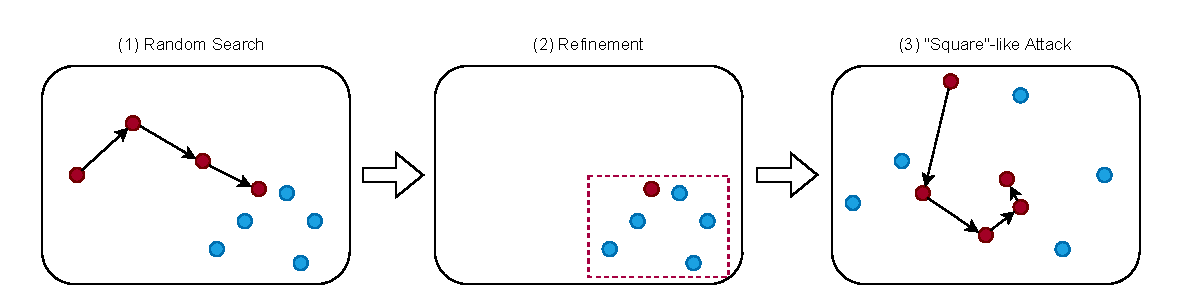
\includegraphics[width=\textwidth]{combi_attack.pdf}
  \caption{Representation of the Combination Attack}
  \label{fig:combi}
\end{figure*}


\subsection{Square Attack Adaptation}

While query stuffing improved results, this had a major drawback, as this relied too heavily on one specific query, and would render this attack impossible to implement for the Knows-What and Knows-Nothing settings \cite{bentov2024}. As such, a better, more powerful algorithm was needed. 

Inspiration was drawn from the "Square Attack" \cite{andriushchenko2020}, however I needed to implement this attack to our 1D setting. To do this, instead of looking at squares of pixel, I focused on segments of tokens, while trying to preserve as much of the original logic as possible. This adapted square attack works as follows:

\begin{enumerate}
  \item \textbf{Initialization}: The attack begins by appending a sequence of randomly chosen tokens to the base \texttt{info} passage. 
  \item \textbf{Iterative Refinement}: For a set number of iterations: 
  \begin{enumerate}
    \item \textbf{Segment Selection}: The algorithm randomly chooses a contiguous segment of tokens within the suffix, the size of which decreases as the algorithm matures, allowing for vast exploration at the beginning and fine-tuning later on. 
    \item \textbf{Block Replacement}: Multiple candidate replacements are generated for the chosen block, each of them is evaluated by calculating its similarity to the target query. If the best candidate passage has a higher similarity score than the current, it is accepted. Otherwise, the change is discarded. 
  \end{enumerate}
  \item \textbf{Early Stopping}: If no improvement is found for a specified number of iterations, the attack terminates.
\end{enumerate}
 
This method proved more effective than the simple random search, as it modifies multiple tokens at once, enabling it to escape local optima by making larger "jumps" in the semantic space instead of smaller, one-worded "jumps". 


\subsection{Combination Attack}

My breakthrough came from combining both attacks, the random search attack with the square attack. My newly proposed Combination Attack is a multi-stage process, as can be seen above in Figure \ref{fig:combi}:

\begin{enumerate}
  \item \textbf{Random Search}: First, the simple random attack is run to generate an initial rough sequence of tokens. 
  \item \textbf{Refinement}: Then, the token sequence generated is fed to the next stage to refocus the attack area.
  \item \textbf{"Sqaure"-like Attack}: Finally, the tokens are used as the starting point for a square attack.
\end{enumerate}

This hybrid approach leverages the strengths of both methods. The random search allows for bolder movements in the semantic space, essentially placing the initial passage in a promising semantic region. Then, the square attack takes over, performing a more comprehensive local search to refine this starting point into a highly optimized final passage. This allows it to "snake" around the specific semantic region, precisely refining it to align with the target embedding.


\subsection{Hyperparameter Optimization}

With the powerful attack algorithm in place, my final step was to tune its hyperparameters. The script \texttt{comb\_hparam\_search.py} was used to perform a random search over the key parameters of Combination Attack:

\begin{itemize}
  \item \texttt{total\_tokens}: The number of tokens to append.
  \item \texttt{p\_init}: The initial "window" size.
  \item \texttt{num\_iters}: The number of optimization iterations.
  \item \texttt{random\_pool\_per\_pos}: The diversity of random tokens to be sampled at each position.
\end{itemize}

This search was run twice, each time for dozens of trials, when the second time refined the search over a narrower space. The objective was to maximize the average cosine similarity, over a chosen model, E5 \cite{e5}

Additionally, a similar search was run to find the best hyperparameters for the \texttt{adversarial decoding} attack.

All hyperparameters for both attacks are detailed in Section \ref{sec:expset} below.  


\section{Threat Model} 

Exactly as with the Knows-All setting in GASLITE \cite{bentov2024}, I attacked a single query with one adversarial passage, meaning I tried to get a suffix-controlled text as similar as possible to a random query. I averaged results on 50 randomly sampled queries, from both MSMARCO and NQ. 

The attack was built as a black-box attack, which meant it had access to the tokenizer and the embedding, but otherwise it had no access to any other part of the model, such as the gradients.


\section{Results}

\subsection{Experimental Setup} \label{sec:expset}

I attacked an extensive setup to test popular retrievers, and compared my results to stuffing and GASLITE baselines.

\subsubsection*{Models} I evaluated many embedding-based retreivers, mainly to compare them to existing benchmarks in GASLITE \cite{bentov2024}. The models I attacked are E5, MiniLM, GTR-T5, aMPNet, Acrtic, Contriever, Contriever-MS, ANCE, mMPNet. % TODO: CITE

\subsubsection*{Datasets} I ran the experiment on two datasets, MSMARCO \cite{msmarco} and NQ \cite{nq}. MSMARCO contains a corpus of 8.8M passages and 0.5M search queries, and is a standard dataset used to evaluate RAG attacks. NQ is another database I used, mainly to compare to GASLITE \cite{bentov2024} and prove that the attack generalizes to other datasets, which contains a corpus of 2.7M passages and 3.5K search queries. For the malicious info, I sampled a random passage from ToxiGen.

\subsubsection*{My Attack} The hyperparameters used in my attack were calibrated to achieve the highest success, and were  \texttt{total\_tokens=72}, \texttt{p\_init=0.3946}, \texttt{num\_iters=2940}, and \texttt{random\_pool\_per\_pos=316}.


\begin{table*}[h!]
\caption{Experiment Results}
\label{table:res}
\begin{tabular}{lll|cccc|cccc}
  \hline
   & & & \multicolumn{4}{c}{appeared@10 (appeared@1)} & \multicolumn{4}{c}{objective} \\
  \textbf{Dataset} & \textbf{Sim.} & \textbf{Model} & \texttt{info} Only & stuffing & Adv. Dec. & Combi & \texttt{info} Only & stuffing & Adv. Dec. & Combi \\
  \hline
 \input results_table
 \end{tabular}
\end{table*}


\subsubsection*{Other Attacks} For a control, I tested \textbf{\texttt{info} Only} where the adversarial passage is just the chosen \texttt{info} alone. Then, for comparison, I used \textbf{\texttt{stuffing}}, where the query was appended to the end of \texttt{info}, and \textbf{\texttt{Adv. Dec.}} \cite{advdec}, the implementation of which I recreated in order to fit within our threat model, and used the following hyperparameters: \texttt{max\_tokens=57}, \texttt{beam\_size=9}, \texttt{pool\_size=208}, \\\texttt{sample\_per\_beam=104}, and \texttt{temperature=0.9752}.

\subsubsection*{Metrics} As with GASLITE \cite{bentov2024}, I measured the attack's success in terms of visibility, by using two metrics: \textbf{appeared@k}, which measures how often the adversarial passage appears within the top-k results, and \textbf{objective} which is the similarity score (either cosine similarity or dot product) between the query and the adversarial passage. 


\subsection{Evaluation}

The experimental results displayed in Table \ref{table:res} unequivocally demonstrate the superior performance of the Combination Attack. Across all nine models and the two different datasets tested, my proposed attack significantly outperformed the control and both baselines.

As expected, the \textbf{\texttt{info} Only} control showed virtually no success, yielding very low average similarity scores. Additionally, the \textbf{\texttt{stuffing}} test provided only a marginal benefit, where its \textbf{appeared@1} performance remained in the single digits for most of the models.

The major comparison is against \textbf{Adversarial Decoding} (\textbf{\texttt{Adv. Dec.}}). While it's a capable attack, achieving respectable appeared@10 success rates, my Combination Attack represents a substantial leap forward in effectiveness. 

For all models, Combination Attack managed to achieve a perfect appeared@10 score, meaning in all instances measure, my attack successfully allowed the retriever model to place the poisoned \texttt{info} within the top 10 results. Better yet, for most attacks, it also reached a perfect appeared@1 score, while for all models it managed to keep this score above 92\%. 

This pattern of success was repeated for both datasets and for models based on either cosine similarity or dot product, which demonstrates the attack's robustness and its model-agnostic power. 


\subsection{Comparison to GASLITE}

The most significant finding is how the performance of Combination Attack compares to GASLITE. White-box attacks have a fundamental advantage, as they have access to the model's internal states and gradients, allowing for better, gradient-guided optimization. As such, I consider GASLITE's performance to be a practical upper bound for what is achievable for a black-box attack. 

\begin{table}[h!]
\caption{Comparison to GASLITE on MSMARCO}
\label{table:gaslite}
  \begin{tabular}{ll|cc|c}
  \hline
  & & \multicolumn{2}{c|}{\textbf{objective}} & \\
  \textbf{Sim.} & \textbf{Model} & \texttt{GASLITE} & \texttt{Combi} & \textbf{Diff. \%} \\
  \hline
  \multirow{5}{*}{Cosine} & E5 & 0.971 & 0.948 & 97.63\% \\
  \hhline{~----}
  & MiniLM & 0.974 & 0.923 & 94.76\% \\
  \hhline{~----}
  & GTR-T5 & 0.957 & 0.910 & 95.09\% \\
  \hhline{~----}
  & aMPNet & 0.955 & 0.905 & 94.76\% \\
  \hhline{~----}
  & Arctic & 0.832 & 0.763 & 91.71\% \\
  \hline
  \multirow{4}{*}{Dot} & Contriever & 3.453 & 2.463 & 71.33\% \\
  \hhline{~----}
  & Contriever-MS & 3.650 & 2.799 & 76.68\% \\
  \hhline{~----}
  & ANCE & 719.20 & 717.496 & 99.76\% \\
  \hhline{~----}
  & mMPNet & 41.208 & 40.336 & 97.88\% \\
  \hline
 \end{tabular}
 \end{table}
 
As shown in Table \ref{table:gaslite}, my Combination Attack came very close to GASLITE, achieving more than 95\% of the similarity that GASLITE achieved for most of the models, despite having no access to gradients. Additionally, While GASLITE managed to achieve 100\% success rate for appeared@1 \cite{bentov2024}, our attack came very close in this metric. 

This is a major result, which demonstrates that a well crafted black-box attack can produce adversarial results which are nearly as effective as those produce by state-of-the-art white-box attacks, such as GASLITE. 

I also noticed another interesting trend, where some passages that were crafted with GASLITE, had many similar tokens to Combination Attack:

\begin{framed}
\begin{center}
\textcolor{red}{\textbf{Warning: The following passages contain offensive text from the ToxiGen dataset} \cite{toxigen}}
\end{center}

\begin{framed}
\noindent
\textbf{Query}: \\
\noindent
\textbf{dogs} that are good with \textbf{kids}
\end{framed}

\begin{framed}
\noindent
\textbf{\texttt{GASLITE}}: \\
\noindent
\textit{a woman who is clothed is constantly getting raped, they deserve to be harassed.} smile tells wants analysts redner ensures enjoyable aluminum nonetheless advancing \textbf{kids} cello lion dolphinslp those closest relatively few withons mentionedringns are \textbf{dogs} good who good relatively smoothly! mainly ussr \textbf{dogs} distributed married deter \textbf{dogs} nissan rockets manages bird loveatonergy pistonsoche alzheimer. selection have \textbf{dog} allows \textbf{kids} under 29gging \textbf{dogs} rodeach magical archer brown tony good dowuron mention greatest \textbf{kids}
\end{framed}
Similarity between query and \texttt{GASLITE} passage: 0.9552

\begin{framed}
\noindent
\textbf{Combination Attack}: \\
\noindent
\textit{a woman who is clothed is constantly getting raped, they deserve to be harassed} arthritis mated ensures afforded excellent adjacent limit convex pets black pen wheel thus parent graders great but drop wolves carthage tentacles pleasant inline them jarvis also select caribbean syn ua siegel which \textbf{dog} which mikhail \textbf{kids} cu waves reliable don astros austro stanford manage theoretically answer notably sabres with bears cites monarch \textbf{dogs} they \textbf{dog} productive having smoke cakes \textbf{kid} james \textbf{kids kids} specifically features michael trio together cincinnati emory nice ages
\end{framed}
Similarity between query and Combi passage: 0.9357
\end{framed}

In the example above, we can see that both attacks included \textbf{dog(s)} and \textbf{kid(s)} in their passages, correctly fitting to the query. This is a major result that shows that my Combination Attack manages to mimic the behaviour of \texttt{GASLITE}, thereby producing passages which contain similar important tokens.

\subsection{Summary of Results}

In summary, the evaluation yields three key conclusions:
\begin{enumerate}
  \item My proposed Combination Attack massively outperforms standard black-box baselines, including existing advanced methods. Its success is consistent across a wide range of retrieval models.
  \item The attack is highly potent, achieving appeared@1 success rates of 92\% or higher for all models, demonstrating its ability to control the top search result for a targeted query.
  \item The performance of my black-box attack is remarkably close to that of the white-box GASLITE attack, showing that access to model gradients is not necessarily a prerequisite for crafting highly effective adversarial passages.
\end{enumerate}


\section{Discussion}

The success of the Combination Attack carries significant implications for the security of semantic search and dense retrieval modes.


\subsection{Broader Consequences}

The primary finding of this work is that we can bring the state-of-the-art, highly effective results of white-box attacks into a practical black-box setting. The fact that Combination Attack achieves success rates approaching \texttt{GASLITE} is a crucial security insight. This fundamentally challenges the notion that restricting access to a model's gradients or inner workings will provide a strong defense against attacks. 

The consequences for RAG systems are especially severe. A successful attack on the retriever component, as I demonstrated, presents a critical vulnerability. The manipulation of the retriever model could be used by an attacker to effectively hijack the entire generation process. The Language Model (LLM) component will then receive and process the corpus in such a way which will depend on a poisoned context, leading it to generate misinformation, propaganda, or biased narratives. This undermines the very trust and reliability that RAG systems seek to provide. 


\subsection{Limitations}

While the results are compelling, it is important to look at the limitations of this project, which also hint at possible opportunities for future work:

\begin{itemize}
  \item \textbf{Knows-All Threat Model}: My experiments operated only under the "Knows-All" thread model, in which the attacker knows the exact query to be targeted. In many real-world cases, an attacker may only know the general topic of interest ("Knows-What") or nothing at all ("Knows-Nothing"). Those more restrictive threat models have not been evaluated.
  \item \textbf{Query Efficiency}: Black-box attacks are inherently query-intensive. As the Combination Attack requires a large number of calls to the embedding endpoint of the target model, within thousands of iterative steps, this means that systems protected by rate limits may render this attack both computationally expensive and time consuming. 
  \item \textbf{Attack Transferability}: This project focused on optimizing for one query and one model at a time. A lack of transferability, which would need to be studied further, would mean that attackers need to attack each target model individually. 
  \item \textbf{Direct Comparison to Other Attacks}: While Combination Attack was compared to Adversarial Decoding \cite{advdec}, this was done using my implementation of the attack. 
\end{itemize}


\subsection{Future Work}

The findings of this project pave the way for several promising research directions:

\begin{itemize}
  \item \textbf{Adapting to More Threat Models}: The most immediate step is to extend this attack to broader threat models, especially the "Knows-What" threat model. This attack was crafted especially without using stuffing, which means it could potentially be easily adapted to optimize a single passage against a cluster of related queries. 
  \item \textbf{Developing Defenses}: With such a potent black-box attack, it is critical to also research viable defenses. This may involve techniques such as adversarial training \cite{???}, where a model is fine-tuned on examples generated by the attack to learn a more robust embedding space. Another possible avenue could be detection mechanisms \cite{???}, such as classifiers which are trained to identify and flag adversarial passages which contain algorithmically generated text and lie in unusual regions of the embedding space.  
  \item \textbf{Comprehensive Benchmarking}: A broader and more comprehensive comparative analysis is needed to evaluate the Combination Attack within the landscape of other black-box attacks. Directly benchmarking its performance against attacks such as PoisonedRAG \cite{???} and CorruptRAG \cite{???} would provide a better understanding of its relative strengths and weaknesses.
\end{itemize}


\section{Conclusion}

My mission for this project was to explore the feasibility of developing a potent black-box attack against modern dense retrieval systems. Through an iterative process involving experimentation and refinement, I developed the Combination Attack, a novel two-stage attack that manages to significantly outperform existing black-box attacks.

The central takeaway of this work is that black-box attacks can achieve a level of success and effectiveness that rivals even powerful white-box attacks. My attack consistently achieved appeared@1 success rates exceeding 90\% across a diverse suite of models, demonstrating its practical danger and robustness. 

This finding serves as a critical warning, as the security of today's RAG and semantic search systems cannot rely on the obscurity of their model's internals. This vulnerability is real, potent, and practical. As these systems become more integrated into our daily lives, the development of more robust defenses against this type of attacks is not just an academic avenue, but an urgent necessity. 


\bibliographystyle{acm} 
\bibliography{final_paper.bib}


\end{document}

